% #############################################################################
% This is Appendix Accessory Information (CHI 2023)
% !TEX root = main.tex
% #############################################################################
\chapter{Accessory Information}
\label{chap:app005}

In this appendix, we provide additional details from Chapter~\ref{chap:chap006} on the use of \ac{AI} models in our \ac{UI}, as well as the severity classification during patient diagnosis, our patient selection, and information about participants.
We also discuss the existing system, evaluating performance recognition, thresholds, and strategies for curating patients, the following steps for explanations and tone, and the repositories.
As follows, we will provide further information to understand the details of our work better.

\section{Extended Motivation}
\label{sec:app005001}

\ac{AI} systems are showing increasing promise for numerous healthcare applications.
Recently, the advantages of \ac{DL} are spawning \ac{AI} systems with human-like performance in several clinical domains~\cite{CALISTO2022102285, Hannun2019, Ruamviboonsuk2019, Stephansen2018}.
However, these applications are not designed to capture the variability of personal or subpopulation level of clinicians~\cite{Uddin2019}.
Recent works highlight how \ac{AI} and the advancement of technologies together are empowering the aim of personalized and precision medicine~\cite{Subramanian2020, HO2020497, Wetzstein2020}.
Given the need to personalize and customize the \ac{AI} recommendations, an essential question in the design of \ac{AI} systems is how they should communicate, considering the professional experience of the clinician.

To achieve a more persuasive and reliable intelligent agent, we must analyze and collect data regarding the clinician's behavior~\cite{PELAU2021106855}.
Communication is essential to increase the reliability of an intelligent agent~\cite{10.1145/3311350.3347162} providing a diagnosis to a clinician.
One way to achieve that is by aligning the levels of assertiveness~\cite{pacheco2019alignment} of the agent with the years of experience of the clinician.
Besides that, explaining `how' and `why' the \ac{AI} assistant achieved a particular output increases trust in the system, solving a problem known as the ``black-box'' problem~\cite{10.1145/3491102.3502104, CALISTO2021102607}.

In this appendix, we present further details of our study for applying {\it BreastScreening-AI} (Section~\ref{sec:sec009004}) in two conditions, where clinicians will interact with conventional and assertiveness-based intelligent agents~\cite{pacheco2019alignment, 10.1145/3311350.3347162}.
The assistant will act as a second reader, resulting in improvements in diagnostic performance, by reducing \acp{FP} and \acp{FN} ({\it i.e.}, Over-Diagnosis {\it vs} Under-Diagnosis), as well as inefficiency and efficacy in the clinical workflow (Section~\ref{sec:sec009005}).
While considerable work has focused on improving the accuracy of \ac{AI} algorithms, comparatively less work focused on improving the adoption and usability of interactive assistance techniques.
This paper broadly examines what clinicians need when using \ac{AI}-powered assistance, the practices they adopt while using diagnostic tools, and how these tools affect end-user attitudes toward the underlying \ac{AI} algorithms.

Here, we detail a within-subject study with 52 clinicians who interacted with both conventional and assertiveness-based agents, diagnosing a total of 35 patients from a dataset of 289 patients, out of which 34\% have benign abnormalities, 31\% have malignant abnormalities, and the other 35\% are healthy patients (Section~\ref{sec:sec009001}).
Two different tones were used to communicate the \ac{AI} recommendations in our assertiveness-based agent, from a more suggestive to a more imposing tone.
Moreover, the assertiveness-based agent explained `{\it how}' and `{\it why}' the \ac{AI} algorithms achieved a particular diagnostic by providing human-interpretable clinical arguments for the achieved outputs.

While we used actual \ac{AI} outputs and clinical arguments curated from human clinicians, the \ac{AI} models were trained for classification and segmentation purposes through different architectures~\cite{HANCER2023321}.
Specifically, through a DenseNet model~\cite{8721151} for a multimodal diagnosis of \ac{MG} and \ac{US} images.
Similarly, a 3D ResNet model~\cite{Aldoj2020} was trained to diagnose the \ac{MRI} volumes.
Our findings suggest that explaining the \ac{AI} outputs and clinical arguments by exploring how to adapt the communication through an assertiveness-based agent can benefit \ac{AI} assistance of medical reasoning.

The novelty of this work lies in applying communication theories through \ac{DL} systems to investigate the impact of assertiveness-based \ac{AI} mediation on different expertise levels in critical medical decision-making.
To achieve this, we updated the design of the {\it BreastScreening-AI} framework~\cite{CALISTO2022102285} to examine how assertiveness-based communication influences different expertise levels in clinical scenarios.
Our contributions encompass knowledge in computational interaction approaches, specifically assertiveness-based \ac{AI} mediation in the \ac{HCI} field, as well as insights into designing interactive systems guided by computational principles for the \acs{CHI} community.

\section{Further Contributions}
\label{sec:app005002}

So far, we have provided an extended motivation (Section~\ref{sec:app005001}) with more information to sustain the work under Section~\ref{sec:chap006001} of Chapter~\ref{chap:chap006}.
In this section, we provide further details on the contributions of this work.
The work was published and {\it peer-reviewed}~\cite{10.1145/3544548.3580682} at the \acs{CHI} 2023 conference.

\vspace{0.50mm}

\noindent
In sum, the main contributions of this work are as follows:

\vspace{0.05mm}

\begin{enumerate}
\item We present a novel approach for personalizing and customizing \ac{AI}-assisted medical reasoning, providing evidence that assertiveness-based agents can alter clinical workflows by effectively adapting the communication depending on the categories of medical professional experience.
\item We demonstrate that while explaining the \ac{AI} outputs can enhance medical efficiency, its impact heavily depends on the communication tone ({\it i.e.}, more suggestive or imposing the \ac{AI} recommendations) of the provided clinical arguments.
\item We report our results demonstrating that these assertiveness-based agents can increase the utility of clinical information found and increase user trust in the \ac{AI} recommendations, without a loss in diagnostic performance.
\item We provide design considerations for adapting the communication in \ac{AI}-assisted medical reasoning, laying a foundation for future implementations of intelligent agents better capable of personalizing and customizing explanations.
\end{enumerate}

\vspace{0.05mm}

Across the following sections, we outline related works on the issues of guiding the \ac{HAII} topic, assisting decision-making, going through some examples of \acp{CDSSe} present in the literature~\cite{NAISEH2023102941, 10.1145/3531146.3533193}, and ending on the effects of \ac{AI} communication.
We then introduce the design of our {\it Assertiveness-based BreastScreening-AI} assistant, followed by our research questions, hypotheses, and methods.
Last, we report our quantitative and qualitative findings, as well as conclude with a discussion of design considerations.

\section{Additional Literature}
\label{sec:app005003}

This section covers additional literature from Section~\ref{sec:chap006002} of Chapter~\ref{chap:chap006} on medical imaging system integration, challenges in clinical decision-making, \acp{CDSSe}, and the effects of \ac{AI} communication. The intersection of cognitive psychology, learnability, and context awareness in \ac{HCI} is examined. Personalized and customized algorithmic suggestions based on medical expertise levels are highlighted, along with the impact of \ac{AI} communication on trust and decision-making. The focus is on studying how assertiveness-based \ac{AI} mediation affects clinicians with different levels of expertise.

Medical imaging systems play a crucial role in diagnosing various modalities, such as \ac{MG}, \ac{US}, and \ac{MRI}, by enabling seamless data retrieval~\cite{faraji2019radiologic}.
Integrating these modalities offers opportunities for quantitative imaging and diagnoses, necessitating specialized data handling, post-processing, and visualization methods~\cite{Igarashi:2016:IVS:2984511.2984537}.
In the clinical domain, medical imaging tools assist experts in making more informed decisions, including identifying cancer prognostics using multi-modal data~\cite{IBRAHIM2019438, Tan2023}.

In this section, we provide additional literature from Section~\ref{sec:chap006002} that expands on integrating \ac{CDSSe} into the radiology workflow.
The selected works aim to explore different aspects and expectations, focusing on enhancing medical imaging diagnosis through assertiveness-based interaction.
These studies shed light on the potential benefits and challenges of incorporating assertiveness-based \ac{AI} systems in the clinical setting.

\subsection{Human-AI Interaction}
\label{sec:app005003001}

Intelligent agents need to provide users with, not only results, but also accounting for their behaviors during decision-making~\cite{10.1145/3313831.3376807}.
In the field of \ac{HCI}, the topic of \ac{XAI} contains subjects that intersect cognitive psychology, learnability, and context awareness~\cite{doi:10.1073/pnas.1618211113, doi:10.1080/07370024.2021.1977128}.
Cognitive psychology is a subject focusing more on explanation theory~\cite{10.1093/mind/fzu023}.
For cognitive psychology, Lombrozo~\cite{LOMBROZO2010303} found that cognitive explanations are strongly connected with causality reasoning.
Learnability is an important part of usability~\cite{10.1145/1753326.1753552}.
Here, Abdul~\cite{10.1145/3173574.3174156} summarized topics of learnability related to designing a \ac{XAI} system, such as hints, guidance, and visualizations.
These aspects contribute to the understanding of how intelligent agents can effectively communicate and provide meaningful explanations in decision-making processes.

Explainable context awareness is a simplistic representation of the context to inform users what is obtained and which action will be done by the system~\cite{10.1145/3313831.3376545}.
Dey et al.~\cite{10.1145/1518701.1518832} designed a tailored interface, providing visual and textual explanations following several context-aware rules.
However, research in both \ac{HCI} and \ac{AI} communities is often disconnected between the two fields~\cite{10.1145/3173574.3174156, 10.1145/3313831.3376807}.
There is a research gap that is not crossing nor combine both fields to the interdisciplinary approach of accounting user's different behavioral characteristics (Section~\ref{chap:app003006} of Appendix~\ref{chap:app003}) during decision-making~\cite{10.1145/3173574.3174156}.
Therefore, both \ac{HCI} and \ac{AI} communities need to bridge this gap with further collaboration and investigation for an understanding enhancement of \acp{HAII} in decision-making processes.

\ac{HAII} incorporates human feedback in the model training process to create better \ac{ML} models.
In this thesis, we refer to the topic as \ac{HAII}, which somehow is addressed by Amershi et al.~\cite{10.1145/3290605.3300233} providing a set of design guidelines~\cite{10.1145/3132272.3134111}.
The work of Kocielnik et al.~\cite{Kocielnik:2019:YAI:3290605.3300641} is also addressing the study on the impact of several methods of expectation setting, and others studied the design for specific \ac{HAII} scenarios~\cite{aha2017ai}.
While prior work relies on handcrafted features~\cite{10.1145/3290605.3300233, Kocielnik:2019:YAI:3290605.3300641}, our approach leverages rich image data features automatically learned from \ac{DL} algorithms by adapting the outcomes to the {\it end-user}.
Specifically, we focus on personalized and customized \ac{AI} suggestions tailored to varying levels of medical expertise.

Many researchers have argued that \ac{HAII} would be improved if the \ac{AI} systems could {\it explain their reasoning}~\cite{10.1145/3411764.3445717, Rudin2022, Kawamleh2022}.
In medicine, explaining predictions from \ac{AI} models is particularly salient, where the uncovered patterns of the model can be more important than prediction performance~\cite{Lundberg2020}.
Lundberg et al.~\cite{Lundberg2018} demonstrate how to retain interpretability by developing a method to provide explanations of model predictions.
Although these works explore how clinicians interact with \ac{AI} recommendations and their perceptions of \ac{AI} outcomes, they are not taking into account cognitive bias in decision-making.
One of the most notorious cognitive differences is seen between people with different levels of expertise and knowledge~\cite{https://doi.org/10.1111/nuf.12430, Seidel2021}.
We are studying how assertiveness-based agents are designed to adapt their communication tone based on expertise levels to reduce cognitive bias.

\subsection{Assisting Clinical Decision-Making}
\label{sec:app005003002}

Although the research in interaction with intelligent agents is recent~\cite{burr2018analysis}, still this topic has seen new advances, {\it e.g.}, chat-bots and other agents~\cite{miller2019intrinsically}.
Recent advances in medical technologies that promote data generation have continued to drive interaction research in the clinical domain~\cite{azuaje2019artificial, Lopes:2017:UHC:3143820.3144118}.
Moreover, the new interest of the medical community to support \ac{AI} research projects and the available public {\it datasets}, are encouraging researchers to work in both fields~\cite{lau2018dataset}.
Therefore, we bring together both \ac{HCI} and \ac{AI} communities to leverage the high-stakes of clinical decision-making.

The introduction of technology for assisting clinical decision-making is fraught with challenges and unintended consequences, such as critical decisions dealing with patient safety, clinician fatigue, and increased medical errors~\cite{10.1093/jamia/ocab291, 10.1117/12.2613082, doi:10.1148/radiol.212631}.
Moreover, clinicians find \ac{AI} systems challenging to use because they may have limited technical skills for adopting these novel technologies, where these technologies are not customized to the behavioral aspects of clinicians~\cite{CALISTO2022102922}.
The \ac{AI} outcomes are challenging to understand and communicate to clinicians, as these systems often have poorly designed interfaces~\cite{10.1145/3555157}, without considering differences in clinician's characteristics during decision-making.
For instance, the reasoning of a novice clinician varies from an expert~\cite{Edgar2022}.

There is a lack of large-scale deployment of these systems in healthcare~\cite{10.1145/3411764.3445432, SU202328, ZAPPATORE20231}, making it difficult to understand how these systems are perceived and used by their intended users in real-world settings.
\ac{HCI} has proposed and conceptualized several approaches to human-AI relationships, such as \ac{iML}~\cite{10.1145/604045.604056}, \ac{HITL}~\cite{holzinger2016interactive, 10.1145/3397481.3450668}, human-\ac{AI} symbiosis~\cite{JARRAHI2018577}, and human-\ac{AI} collaboration~\cite{10.1145/3411764.3445432}.
However, these approaches mainly use human input to improve the prediction accuracy, model efficiency, and interpretability of \ac{AI} to the unwanted added burdens on healthcare professionals~\cite{10.1145/3555157, 10.1145/3209889.3209897}.
Wang et al.~\cite{10.1145/3411764.3445432} studied the perception and usage of \ac{AI} systems for assisting clinical decision-making, but the work is not accounting the potential differences between behavioral reasoning.
Similarly, the work of Panigutti et al.~\cite{10.1145/3491102.3502104} is only considering accurate algorithmic suggestions without considering the clinician's professional medical experience.

In conclusion, integrating \ac{AI} systems into clinical decision-making requires a holistic approach that considers not only the technical challenges but also the unique behavioral characteristics and professional expertise of clinicians.
The collaboration between \ac{HCI} and \ac{AI} communities is crucial in developing intelligent systems that are user-friendly, personalized, and effective in real-world healthcare settings.
By bridging the gaps between these disciplines and understanding the complex interactions between humans and \ac{AI}, we can ensure that \ac{AI} technologies in healthcare are designed to meet the specific needs of clinicians, ultimately leading to improved patient outcomes.
In our work, we contribute to addressing these literature gaps by focusing on the personalization and customization of algorithmic suggestions based on different levels of professional medical experience.

\subsection{Clinical Decision Support Systems}
\label{sec:app005003003}

In medical applications, \ac{DL} systems have also been the major contributor to the success of several \ac{CDSSe} applications~\cite{esteva2019guide}.
Such \ac{CDSSe} applications can detect and learn patterns or make predictions to assist clinicians, such as pathologists, or radiologists, among others, in high-stakes clinical decision-making~\cite{10.1145/3555157}.
For instance, on the diagnosis of skin cancer~\cite{esteva2017dermatologist}, the segmentation of cardiac \ac{MRI}~\cite{8759179}, or breast cancer detection~\cite{MAICAS2019101562}, there are a variety of works where \ac{DL} systems were introduced for clinical purposes.
Their outstanding performance in identifying meaningful patterns within the available data was recently used to help humans learn new biomarkers of specific diseases~\cite{wang2019deep}.
Because of that, several works are arguing that these models can see beyond what a trained radiologist sees in medical images~\cite{mckinney2020international, Rajpurkar2022, MAIERHEIN2022102306}.
Although some works are already contemplating the idea of a \ac{CDSSe} that predicts and explains some \ac{AI} outcomes~\cite{MAICAS2019101562, CALISTO2022102285}, they ignore the need to adapt the communication tone for personalized and customized medicine.

Most of the best-performing \acp{CDSSe} rely on \ac{ML} algorithms that learn specific tasks from training data~\cite{10.1001/jama.2018.17163, Zaman49, 10.1145/3399715.3399744}.
The field recently gained enormous interest, primarily due to the practical successes of \ac{DL}~\cite{10.1007/978-3-030-22871-2_67}.
The rapid and widespread development of \ac{DL} methods supports a wide range of image analysis tasks in breast cancer diagnosis, including classification, detection, and segmentation \cite{lecun2015deep, DIN2022106073}.
These methods rely on large annotated datasets to learn essential and discriminative image features for each specific task, with performances matching and even surpassing humans \cite{esteva2017dermatologist}.
However, past works highlight several obstacles in going from research and development environments to the hospital or real clinical settings for these set of applications~\cite{https://doi.org/10.3322/caac.21552, 10.1145/3313831.3376718}.

The lack of utility to clinicians and logistical hurdles that slow or block deployment are frequent obstacles in real clinical settings~\cite{Elwyn2013, Musen2021}.
Even systems with widespread adoption, such as systems to aid radiologists during breast cancer diagnosis, require them to do more work~\cite{KOHLI2018535}.
Instead of reducing the radiologist workload or easing the clinical workflow, these systems are generally not improving the radiologist's diagnostic accuracy~\cite{Cole2014fi, KOHLI2018535}.

The work of Beede et al.~\cite{10.1145/3313831.3376718} studies the introduction of \ac{CDSSe} set of tools, primarily focusing on \ac{AI} systems that use clinical data.
However, they are not examining the use of real patient \ac{AI} predictions.
Our work covers this gap by, not only, incorporating real granular patient information from the \ac{AI} outputs, but also studying how to personalize and customize a \ac{CDSSe} for the clinical setting.

Across the \ac{HCI} literature~\cite{10.1145/3311957.3359433, 10.1145/3359206, Fitzpatrick2013, 10.1145/3538882.3542790}, or more precisely, from the \acs{CHI} community~\cite{10.1145/3313831.3376718, 10.1145/3290605.3300234}, human-centered evaluation of interactive, \ac{DL} systems, is an open area of research within clinical environments.
Cai et al.~\cite{10.1145/3290605.3300234} created interactive techniques, leading to an increased diagnostic utility and user trust in the predictions from a \ac{DL} system, used by clinicians in a lab setting.
Correspondingly, Cai et al.~\cite{10.1145/3359206} examined in the lab setting what information clinicians found to be important when being introduced to \ac{AI} assistants, before integrating these assistants into routine prostate cancer screening practice.
While these works bring us closer to understanding the clinician's needs as they interact with \ac{DL}-based systems, they do not account for the heterogeneous behavioral nature of decision-making.

\subsection{Effects of AI Communication}
\label{sec:app005003004}

Trust is critical in communication (Section~\ref{chap:app003005002} of Appendix~\ref{chap:app003}), especially, in clinical environments, where clinicians are exposed to critical scenarios that affect life decisions~\cite{Amann2020}.
From the \ac{HCI} literature~\cite{10.1145/3479587, 10.1145/3334480.3375147, 10.1145/3334480.3382842}, we know that the development of trust is influenced by the positive motivational attribution between the communication entity and the user.
The work of Hohenstein et al.~\cite{HOHENSTEIN2020106190} is showing that a successful collaboration between humans and \ac{AI} occurs when ambiguity and uncertainty in terms of perceptions are reduced through trust~\cite{HOHENSTEIN2020106190}.
While communicating \ac{AI} predictions and explanations is shaping the design of recent works~\cite{Lundberg2020, 10.1145/1518701.1518832}, we do not know how assertiveness-based \ac{AI} mediation is affecting novice or expert clinicians.

To avoid unexpected clinical consequences, we need to understand the effects of \ac{AI} communication on human interactions.
In fact, the direct effects of communication are suggesting that clinicians' level of trust in an \ac{AI} system directly affects their perception of the outcomes~\cite{HOHENSTEIN2020106190}.
Panigutti et al.~\cite{10.1145/3491102.3502104} are arguing that higher levels of trust will cause the clinician to have a positive attitude, resulting in high satisfaction and positive perceptions of performance with respect to the interaction outcome.
Moderation via adapting the communication suggests that trust will influence how a clinician interprets and evaluates information relevant to attitude and behavior.
Attribution theory tells us that when behavior is consistent with explanations, humans will attribute causality to self characteristics and needs~\cite{LOMBROZO2010303}.
On the other hand, when behavior is inconsistent with prior expectations, where there is missing information or ambiguity, external cues will determine behavior~\cite{HOHENSTEIN2020106190}.
As an example, a novice clinician asking for help and receiving a suggestive, {\it i.e.}, non-assertive communication.
During a human-human interaction, a novice clinician would receive an assertive recommendation from an expert advisor.
The novelty of our work lies in applying assertive communication theories in a deep learning system and clinical scenario.

\section{Assertiveness-based System Details}
\label{sec:app005004}

In this section, we provide further details of the system that were summarized in Section~\ref{sec:chap006003} of Chapter~\ref{chap:chap006}.
Clinicians can open the patient by selecting the ID in a list of patients.
When the patient is open (attribute 1 of Figure~\ref{fig:fig096}), clinicians can select each respective image of the breast, by dragging-drop each image to the view-ports.
From here, clinicians can manipulate the image through the toolbox (attribute 3 of Figure~\ref{fig:fig096}).
In the end, the idea is to {\it accept} or {\it reject} the final recommendation of the AI agent (attribute 5 of Figure~\ref{fig:fig096}), while clinicians can also ask for an {\it explanation} to support their final decision-making.
The key difference between the two AI agents was in how they show communication with clinicians.
A typical output from an AI model includes not only the predicted classification of the BIRADS, but also a likelihood distribution over all possible classification choices.

In our study, both AI agents were designed to communicate this type of {\it quantitative} confidence in two ways (Figure~\ref{fig:fig098}):
(1) for the conventional condition, clinicians could simply see the suggested numeric representation of the BIRADS and the respective accuracy of the model;
(2) for the assertiveness-based condition, the agent was communicating the clinical arguments along with the communication of the BIRADS and accuracy, but this time by descriptive information.
While our conventional agent employed this baseline numeric representation of confidence, our assertiveness-based agent is communicating the {\it quantitative} confidence based on a descriptive sentence of the clinical arguments.
Specifically, the image view-port was augmented with an additional bounding box or circle ellipse {\bf highlighting the lesion characteristics} that were likely to explain the final BIRADS classification.
Note that these suggestions did not dictate the order in which imaging modalities are presented to clinicians.
Indeed, clinicians can remain to decide freely what modalities and clinical arguments are reviewed first.

%%%%%%%%%%%%%%%%%%%%%%%%%%%%%%%%%%%%%%%%%%%%%%%%%%%
\begin{figure}[htpb]
\begin{center}
\centering
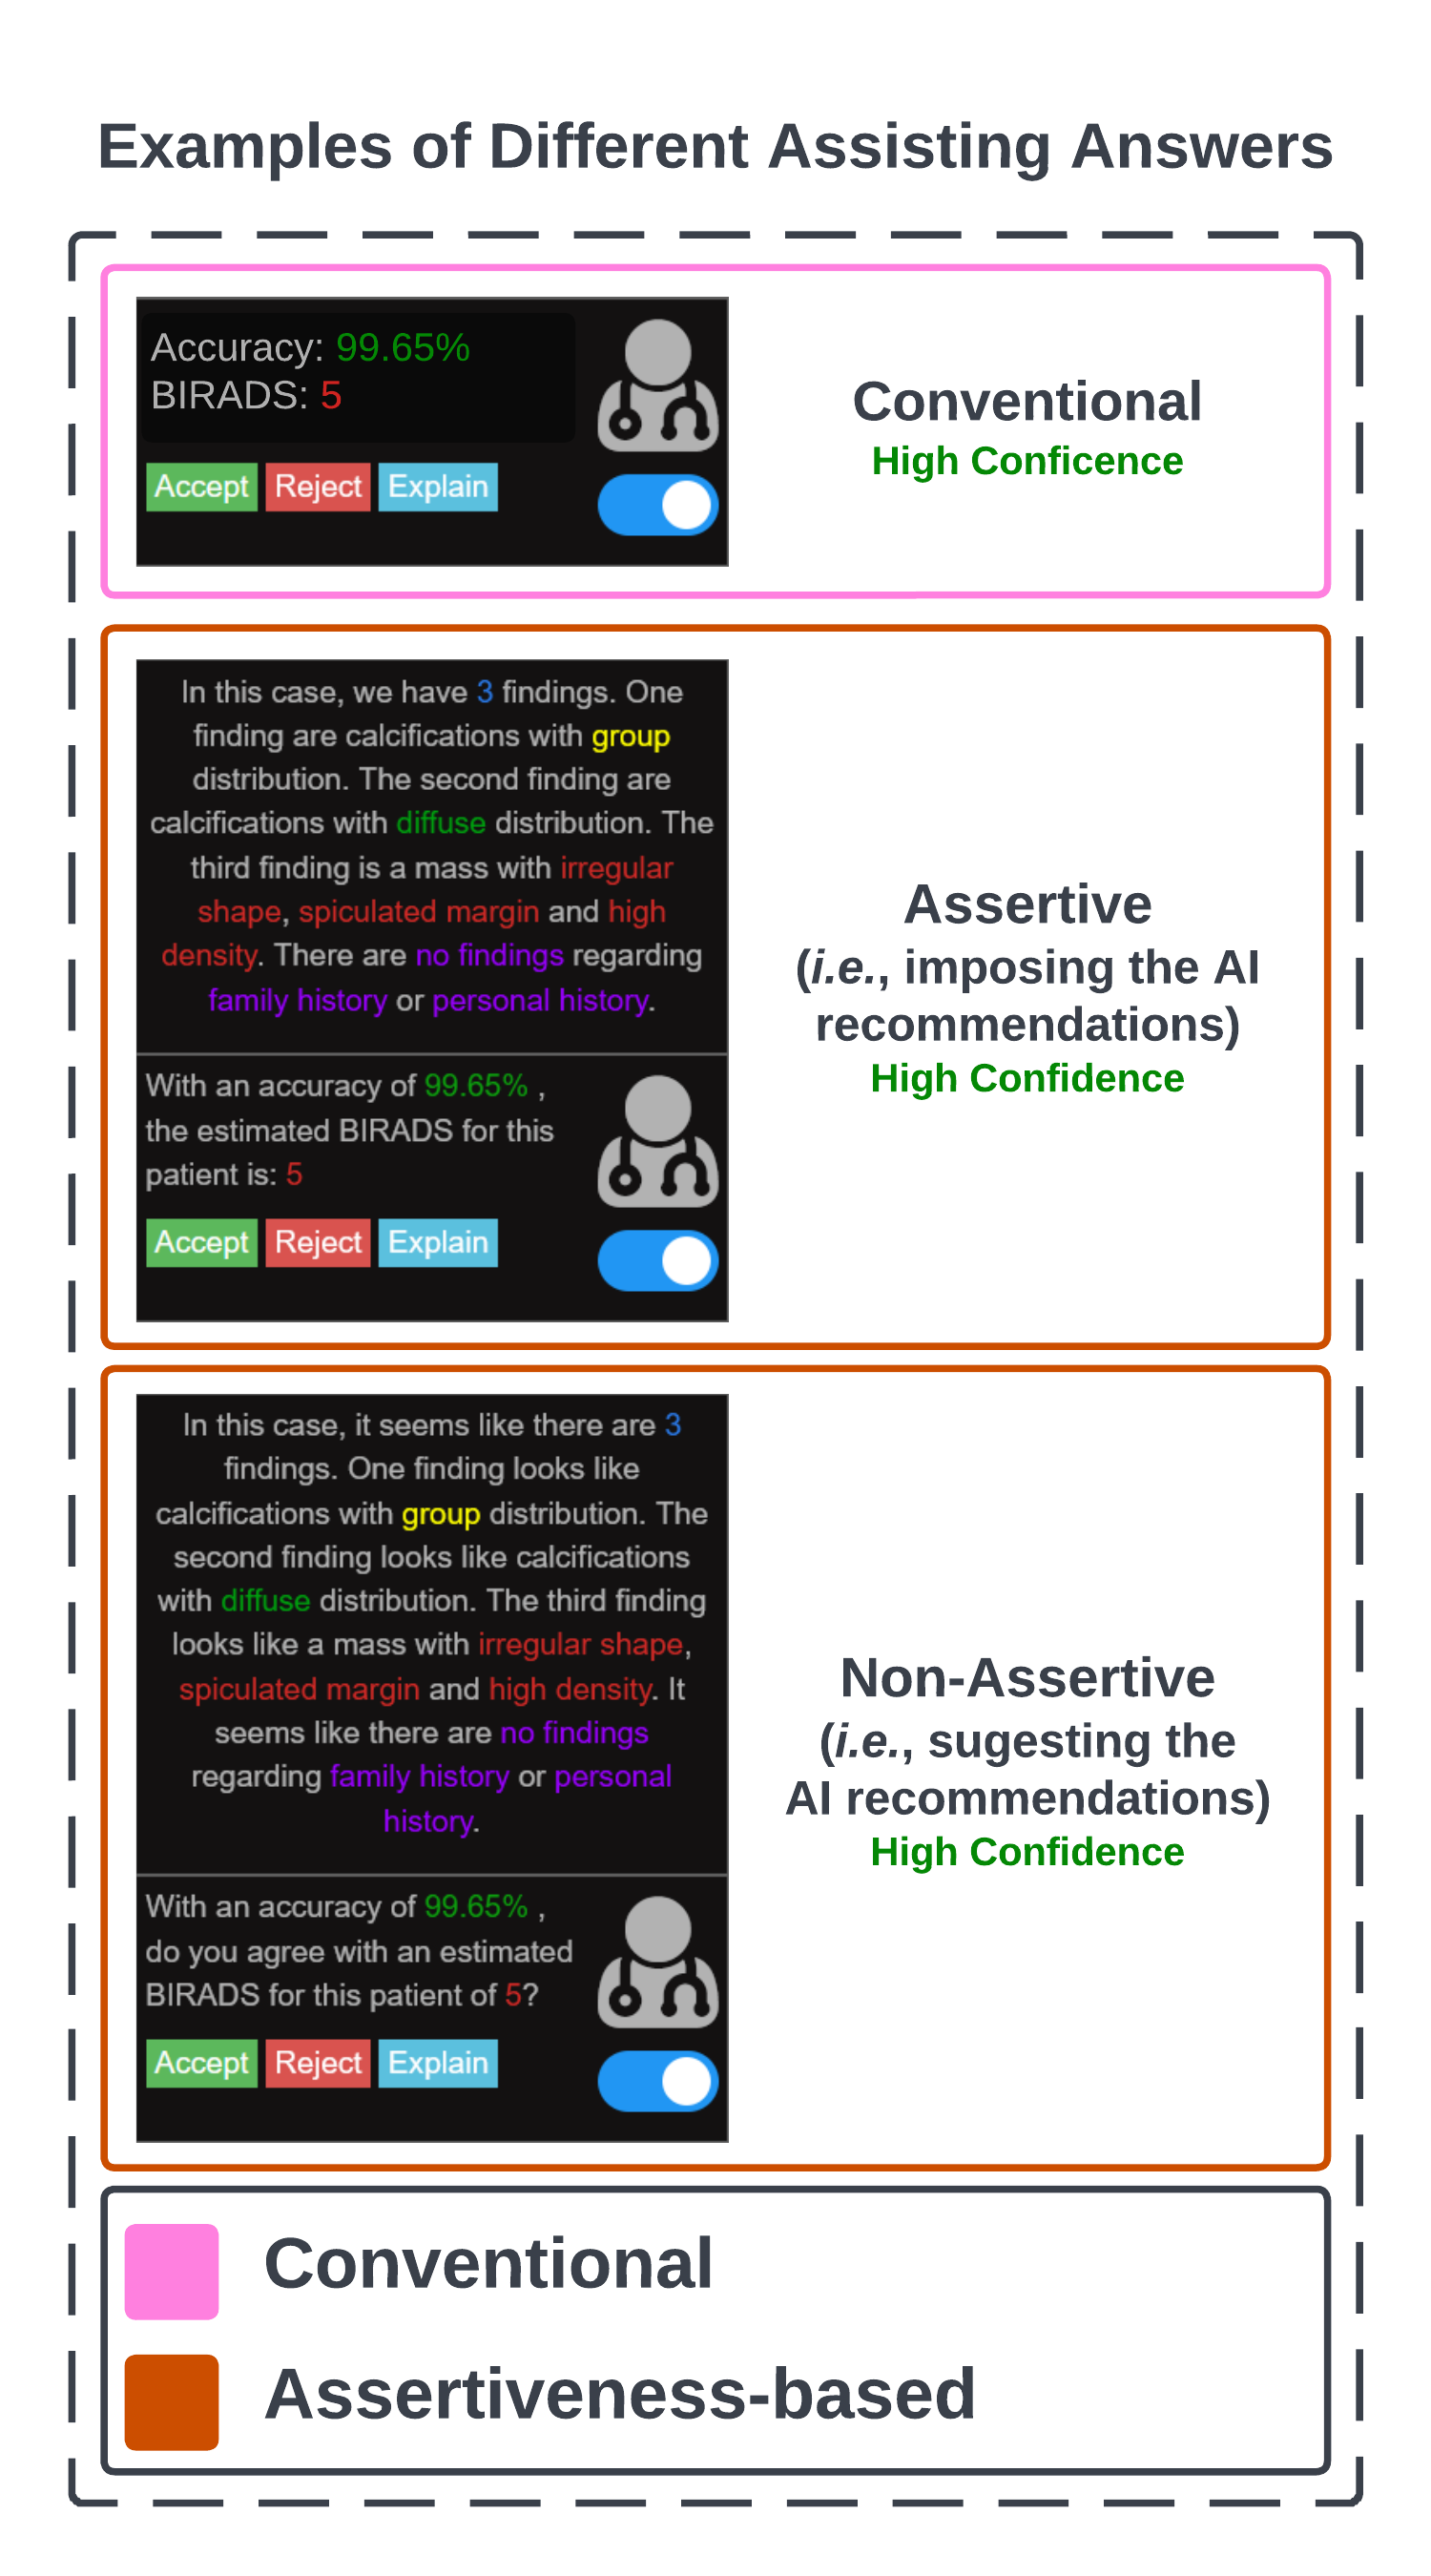
\includegraphics[width=0.625\textwidth]{fig098}
\end{center}
\caption[]{Example of representative use cases for the different testing trials. From top to the bottom, the first agent is representing a conventional example (pink), while the other two are representing assertiveness-based examples (brown), from assertive to non-assertive communication.}
\label{fig:fig098}
\end{figure}
%%%%%%%%%%%%%%%%%%%%%%%%%%%%%%%%%%%%%%%%%%%%%%%%%%%

The patient's detailed augmentation for medical imaging on breast cancer diagnosis was extended with an {\bf assertiveness-based explanation}.
With our system, we are listing human-interpretable clinical arguments for classification and segmentation recommendations that would adapt their communication depending on the personalized and customized demographic characteristics of the clinician.
These clinical arguments correspond to the classification outputs of an AI model and were trained on data (Section~\ref{sec:chap006005002}) from real-world clinical cases, as described next.










\section{Severity Classification}
\label{sec:app00100X}

\ac{BI-RADS} stands for ``{\it Breast Imaging Reporting and Data System}'' and is a system used to standardize the way in which radiologists report the findings of mammograms and other imaging exams of the breast~\cite{SPAK2017179, mckinney2020international}.
The \ac{BI-RADS} provides a standardized method for reporting the results of breast imaging exams, which can help to ensure that the information is accurate and consistent.
As a quantitative approach, it serves for representing the severity assessment of patients with breast imaging exams.
This information is helpful as an input for \ac{AI} models that are designed to assist with diagnosing breast cancer, as it provides a standardized way of representing the findings of imaging exams~\cite{MAICAS2019101562}.

By using the \ac{BI-RADS} system as an input for \ac{AI} models, it may be possible to improve the accuracy and reliability of the model's predictions, and to help prevent bias in the results.
The \ac{BI-RADS} system uses a scale from {\bf 0} to {\bf 6} for categorizing the findings of breast imaging exams.
However, in our study we just considered the scale from {\bf 1} to {\bf 5}, as the {\bf 0} means that the case is inconclusive, where we need to acquire more images, and {\bf 6} means we already have biopsy confirmation by previously known lesion.

\vspace{1.5mm}

\noindent
Here is a brief overview of each category on the \ac{BI-RADS} scale:

\vspace{0.5mm}

\begin{enumerate}
\item {\bf Negative:} The exam did not show any abnormalities and the patient's breast tissue appears normal.
\item {\bf Benign Finding:} The exam showed a benign (non-cancerous) abnormality in the breast tissue.
\item {\bf Probably Benign:} The exam showed an abnormality that is likely to be benign, but further testing may be needed to confirm this.
\item {\bf Suspicious Abnormality:} The exam showed an abnormality that is suspicious for cancer and further testing, such as a biopsy, is needed to determine if it is cancerous.
\item {\bf Highly Suggestive of Cancer:} The exam showed an abnormality that is highly suggestive of cancer, and a biopsy is recommended to confirm the diagnosis.
\end{enumerate}

\vspace{0.5mm}

It is important to note that the \ac{BI-RADS} score is only a tool for reporting the results of breast imaging exams and does not provide a definitive diagnosis of cancer.
A biopsy is usually needed to confirm a cancer diagnosis.
For more details, follow the \href{https://radiopaedia.org/articles/breast-imaging-reporting-and-data-system-bi-rads}{link} (\href{https://radiopaedia.org/articles/breast-imaging-reporting-and-data-system-bi-rads}{radiopaedia.org/articles/breast-imaging-reporting-and-data-system-bi-rads}).
Accessed on the 11th of January 2023.

\section{Patient Selection}
\label{sec:app001002}

In Chapter~\ref{chap:chap006}, we used a total of 338 cases and acquired in the \ac{HFF} clinical institution.
From this set of 338 cases, 289 were classified by the head of radiology.
Each patient has several images concerning four X-ray \ac{MG} modalities (two in \ac{CC} and two \ac{MLO} views), one or two US images, and roughly 5 volumes in \ac{MRI}.
In the \ac{MRI} volumes, we take numerous image slices per patient, where the lesion is present.

From the 289 classified cases, we selected a total of 35 patients to be classified by our \ac{AI} models.
Because we aim to test the three trials ({\it i.e.}, conventional {\it vs.} non-assertive {\it vs.} assertive), plus the two groups of medical professional experience ({\it i.e.}, novice {\it vs.} expert) we computed at least $2^5=32$ the number of patients.
Hence, the 35 patients were selected to cover that magnitude of patients.
This classification corresponds to assigning a \ac{BI-RADS} value for each modality image of the exam.

\section{Participants Information}
\label{sec:app001003}

In this study, we collected information about the participants through an initial survey, and this included details about their gender, age, geographic location, and professional experience (Table~\ref{tab:tab015}).
Additionally, we also ask participants about their professional background, in reading medical imaging data.
Regarding the professional background, 11.54\% of participants are doing their medical internships, 3.85\% were breast medical surgeons, but with knowledge of reading medical images, and 84.61\% were medical radiologists, reading and diagnosing patients every day.

%%%%%%%%%%%%%%%%%%%%%%%%%%%%%%%%%%%%%%%%%%%%%%%%%%%
% Please add the following required packages to your document preamble:
% \usepackage{multirow}
\begin{table}[htpb]
\centering
\resizebox{\columnwidth}{!}{%
\begin{tabular}{|c|c|c|c|}
\hline
Demographic                           & Group           & Frequency & Percentage \\ \hline
\multirow{2}{*}{Gender}               & Female          & 36        & 69.23\%    \\ \cline{2-4} 
                                      & Male            & 16        & 30.76\%    \\ \hline
\multirow{5}{*}{Age}                  & 18 - 29         & 11        & 21.15\%    \\ \cline{2-4} 
                                      & 30 - 39         & 12        & 23.08\%    \\ \cline{2-4} 
                                      & 40 - 49         & 10        & 19.23\%    \\ \cline{2-4} 
                                      & 50 - 59         & 10        & 19.23\%    \\ \cline{2-4} 
                                      & \textgreater 59 & 9         & 17.31\%    \\ \hline
\multirow{11}{*}{Geographic Location} & Hospital 1      & 15        & 28.85\%    \\ \cline{2-4} 
                                      & Hospital 2      & 12        & 23.08\%    \\ \cline{2-4} 
                                      & Hospital 3      & 2         & 3.85\%     \\ \cline{2-4} 
                                      & Hospital 4      & 9         & 17.31\%    \\ \cline{2-4} 
                                      & Hospital 5      & 1         & 1.91\%     \\ \cline{2-4} 
                                      & Hospital 6      & 1         & 1.91\%     \\ \cline{2-4} 
                                      & Hospital 7      & 6         & 11.54\%    \\ \cline{2-4} 
                                      & Hospital 8      & 1         & 1.91\%     \\ \cline{2-4} 
                                      & Hospital 9      & 1         & 1.91\%     \\ \cline{2-4} 
                                      & Hospital 10     & 1         & 1.91\%     \\ 
                                      \cline{2-4} 
                                      & Hospital 11     & 3         & 5.77\%     \\ \hline
\multirow{4}{*}{Medical Experience}   & Interns         & 6         & 11.54\%    \\ \cline{2-4} 
                                      & Juniors         & 17        & 32.69\%    \\ \cline{2-4} 
                                      & Middles         & 11        & 21.15\%    \\ \cline{2-4} 
                                      & Seniors         & 18        & 34.62\%    \\ \hline
\end{tabular}
}
\caption[]{Characteristics of participants for demographic groups with frequency and percentage. The main characteristics are gender, age, geographic location (clinical institution), and medical experience.}
\label{tab:tab015}
\end{table}
%%%%%%%%%%%%%%%%%%%%%%%%%%%%%%%%%%%%%%%%%%%%%%%%%%%

\section{Existing System}
\label{sec:app001004}

Our new approach allows for a more flexible and dynamic system.
Furthermore, the new system addresses some limitations of the traditional system~\cite{CALISTO2022102285}, providing a more robust and scalable solution.
Ultimately, offering a new and innovative approach for solving the diagnostic task.

The \ac{AI} models in this study are not fusing the predictions from different imaging modalities ({\it e.g.}, \ac{MG}, \ac{US}, or \ac{MRI}).
Instead, each modality had its own ground-truth score, which refers to the correct or known diagnosis for a given patient.
This is because the different modalities may provide different information about a patient's breast tissue, and may, therefore; result in different diagnoses and \ac{BI-RADS} scores for a given patient.
Hence, the \ac{AI} models in this study generated individual final predictions for each modality.

Specifically, the DenseNet model~\cite{8721151} was used to estimate the lesion score for 2D imaging data, such as \ac{MG} and \ac{US} images.
The 3D ResNet model~\cite{Aldoj2020} was used to estimate the lesion score for 3D data, such as \ac{MRI} volumes.
Lesion score refers to the likelihood that a specific area of the breast tissue is cancerous, and is typically used as part of the \ac{BI-RADS} score for reporting the results of exams.

\section{Evaluating Performance Recognition}
\label{sec:app001005}

We have used the false-positive and false-negative metrics for evaluating the performance of recognition of clinicians, since these metrics are straightforwardly obtained from a classification process.
We chose to use these metrics because they are widely recognized as important indicators of performance in medical imaging classification tasks.
Particularly, in the context of breast cancer diagnosis, where false-positives and false-negatives can have significant consequences for patient care.
Furthermore, we believe that these metrics provide a more balanced and comprehensive evaluation of performance than classification accuracy, which can be misleading in imbalanced datasets.
For instance, if a clinician provides a \ac{BI-RADS} of 3 but the real \ac{BI-RADS} is a 5, we consider it as a false-negative result.
On the other hand, if the real \ac{BI-RADS} is a 2, but the clinician provides a \ac{BI-RADS} of 4, we consider it as a false-positive.
Where the ``real'' score is the ground-truth provided by the expert from the \ac{HFF} clinical institution.

Overall, our goal was to evaluate the performance of our system in terms of its ability to reduce false-positives and false-negatives.
We found that our classifiers achieved an average decrease of about 26\% for the false-positive rate and about 2\% for the false-negative rate, outperforming previous approaches that have been proposed for this task~\cite{CALISTO2022102285}.
Moreover, we believe that the false-positive and false-negative metrics we used are appropriate for this purpose.
By using these metrics, we were able to demonstrate the potential of our \ac{AI}-assisted approach for reducing false-positives and false-negatives, and we believe that our findings could help to inspire future research.

\section{Thresholds \& Strategies for Curating Patients}
\label{sec:app001006}

Similar to what was already described (Section~\ref{sec:app001001}), the rationale is the following.
The \ac{BI-RADS} score ranges from 0-to-6 scale, with the following meaning:
0 -- inconclusive,
1 -- no findings,
2 -- benign findings,
3 -- probably benign,
4 -- suspicious findings,
5 -- high suspicious malignancy,
6 -- previously known lesion.
\ac{BI-RADS} of 0 and 6 are ignored in our study, because they are meaningless for prediction purposes.

\vspace{1.15mm}

\noindent
We have clustered the values above into three classes as follows:

\vspace{0.05mm}

\begin{itemize}
\item ``No Findings'' with \ac{BI-RADS} = 1
\item ``Benign, probably benign findings'' with \ac{BI-RADS} = \{2, 3\}
\item ``Probably, highly suspicious malignancy findings'' with \ac{BI-RADS} = \{4, 5\}
\end{itemize}

Thus, the  DenseNet (for 2D \ac{MG} and \ac{US}) and the ResNet (for 3D \ac{MRI}), three classes for the classification.
We take the values from 1-to-5, since the other two values do not count for the diagnosis.
Notice that both networks are trained with the \ac{BI-RADS} ground truth provided by a radiologist from the \ac{HFF} clinical institution.

\section{Next Steps for Explanations and Tone}
\label{sec:app001007}

In Chapter~\ref{chap:chap006}, we resort to two main classes of tones:
(1) assertive, by having a more authoritative tone, while imposing the \ac{AI} recommendations; and
(2) non-assertive, while being a more suggestive agent.
However, and considering the clinical context, this should be expanded not only to test more trials in a near future, but also to a larger extent of the communication tones.
Concretely, the explanations should be attached to the concept of the lexicon for each breast modalities~\cite{SPAK2017179}.
For instance, having the explanation: ``scattered areas'' (\texttt{lex\_1}), ``fibrogandular density'' (\texttt{lex\_2})  or ``scattered fibroglandular tissue'' (\texttt{lex\_3}), and ``ring enhancement mass'' (\texttt{lex\_4}).
However, we recognize that there may be other communication tones that could be useful in the clinical context, and we plan to explore these in future research.

\vspace{1.5mm}

\noindent
To study the full effects of the style of tone, we will need the following trials:

\vspace{0.05mm}

\begin{enumerate}
\item Conventional Agent;
\item Agent with Explanations in Neutral Tone;
\item Agent with Explanations in Non-Assertive Tone; and
\item Agent with Explanations in Assertive Tone.
\end{enumerate}

\vspace{0.5mm}

This is an interesting point that presently we are pursuing our research in this direction.
By providing more detailed and accurate explanations, we believe that our \ac{AI}-assisted system can improve the diagnostic performance of medical imaging classification in the clinical domain of breast cancer.

\section{Repositories}
\label{sec:app001sec010}

Our repositories are accessible to the public and can be easily located online.
Please follow the \texttt{\href{https://github.com/MIMBCD-UI/prototype-assertive-reactive}{prototype-assertive-reactive}} repository (\href{https://github.com/MIMBCD-UI/prototype-assertive-reactive}{github.com/MIMBCD-UI/prototype-assertive-reactive}) for more details about the source code of the prototypes.
In terms of results and statistical analysis, all information is available in the \texttt{\href{https://github.com/MIMBCD-UI/sa-uta11-results}{sa-uta11-results}} repository (\href{https://github.com/MIMBCD-UI/sa-uta11-results}{github.com/MIMBCD-UI/sa-uta11-results}).
The repositories have the linking pointers for the other related repositories, such as the datasets, source code of the \ac{AI} models, prototypes, documentation, between others.
These links were accessed on the 25th of January 2023.

\section{Intellectual Property}
\label{sec:app001sec011}

The work described in this paper is covered by pending patent applications~\cite{WO2022071818A1}, filed by \href{https://tecnico.ulisboa.pt}{Instituto Superior T\'{e}cnico}.
The contents of this paper are intended to be informative to the scientific and technical community.
They are not intended to be used to limit the scope of the pending patent application.
The patent rights will be enforced to the extent necessary to protect the proprietary interests of the patent holders.
For more information, further details are available in the \texttt{\href{https://github.com/MIMBCD-UI/sa-uta11-results/blob/main/LICENSE.md}{LICENSE.md}} file of the \texttt{\href{https://github.com/MIMBCD-UI/sa-uta11-results}{sa-uta11-results}} repository (\href{https://github.com/MIMBCD-UI/sa-uta11-results}{github.com/MIMBCD-UI/sa-uta11-results}).
Accessed on the 11th of January 2023.

\section{Epilogue}
\label{sec:app001sec013}

In conclusion, this appendix provides additional details from Chapter~\ref{chap:chap006} on key aspects of our work, including the use of \ac{AI} models in the design of our \ac{UI}, patient selection and diagnosis classification, as well as information about study participants.
We have also discussed the evaluation of performance recognition, thresholds, and patient curation strategies in the existing system.
Moving forward, we plan to explore more communication tones and explanations for our \ac{AI}-assisted system, as well as to conduct further trials to better understand their effects on the diagnostic performance of medical imaging classification.
The repositories for our source code and statistical analysis are publicly accessible, and we remind readers that the work is covered by pending patent applications.
We hope that the information presented here will help to advance the field of \ac{AI}-assisted medical imaging diagnosis, and we look forward to further research in this area.